\chapter{Introduction}

\section{Ultrafast Dynamics in Condensed Matter Systems}

timescales and processes in solids

\section{Attosecond Transient Absorption Spectroscopy (ATAS)}

\subsubsection{why are you doing it with HHG?}

include figure of pulse duration vs photon energy, showing different light sources (synchrotrons, HHG sources, XFEL, etc.) tie this into the timescales neccessary to probe condensed matter physics.

\subsection{overview of the technique}

references \cite{ramaseshaRealTimeProbingElectron2016}

The basic concept of an \textit{attosecond transient absorption spectroscopy} (ATAS) experiment is shown in \cref{fig:ATAS_Cartoon_Si_Leone}. In this experiment, a sample is placed at the combined XUV/IR focus in a transmission (normal) geometry. An XUV photon spectrometer is placed behind the sample and the transmitted XUV spectrum $S$ is measured as a function of XUV-IR delay. The IR light is not measured by the spectrometer.

Fundamentally, changes in photoabsorption correspond to electron and phonon dynamics in the sample. In condensed matter materials, these processes occur on the picosecond ($10^{-12}$ s), femtosecond ($10^{-15}$ s) and even attosecond ($10^{-18}$ s) time scales \cite{schultzeAttosecondBandgapDynamics2014,cushingDifferentiatingPhotoexcitedCarrier2019,zurchDirectSimultaneousObservation2017,volkovAttosecondScreeningDynamics2019}. At XUV energies, photons drive electronic transitions from a core-level state to one near the Fermi level, which requires electron population in the initial state and a vacancy in the final state. Because the initial state is tens or even hundreds of eV below the bandgap, it is shielded from the external IR field. The final states, being closer to the Fermi level, enjoy no such shielding. Therefore they can be distorted by the external IR field, and the electron population can be transferred between these states in response to the IR field. After an initial IR excitation, electrons relax via different scattering channels, including with other electrons or phonon modes with longer lifetimes. Provided the dipole selection rules allow it, the photoabsorption spectrum is sensitive to all of these dynamics. Thus by measuring the XUV spectrum as a function of XUV-IR delay, we can track the electronic and phononic response of a sample to an ultrafast IR excitation.


\subsubsection{induced dipole interpretation}

\subsubsection{population transfer and probing interpretation}

\subsubsection{comparison of absorptive and reflective measurements}


\begin{figure}
	\centering
	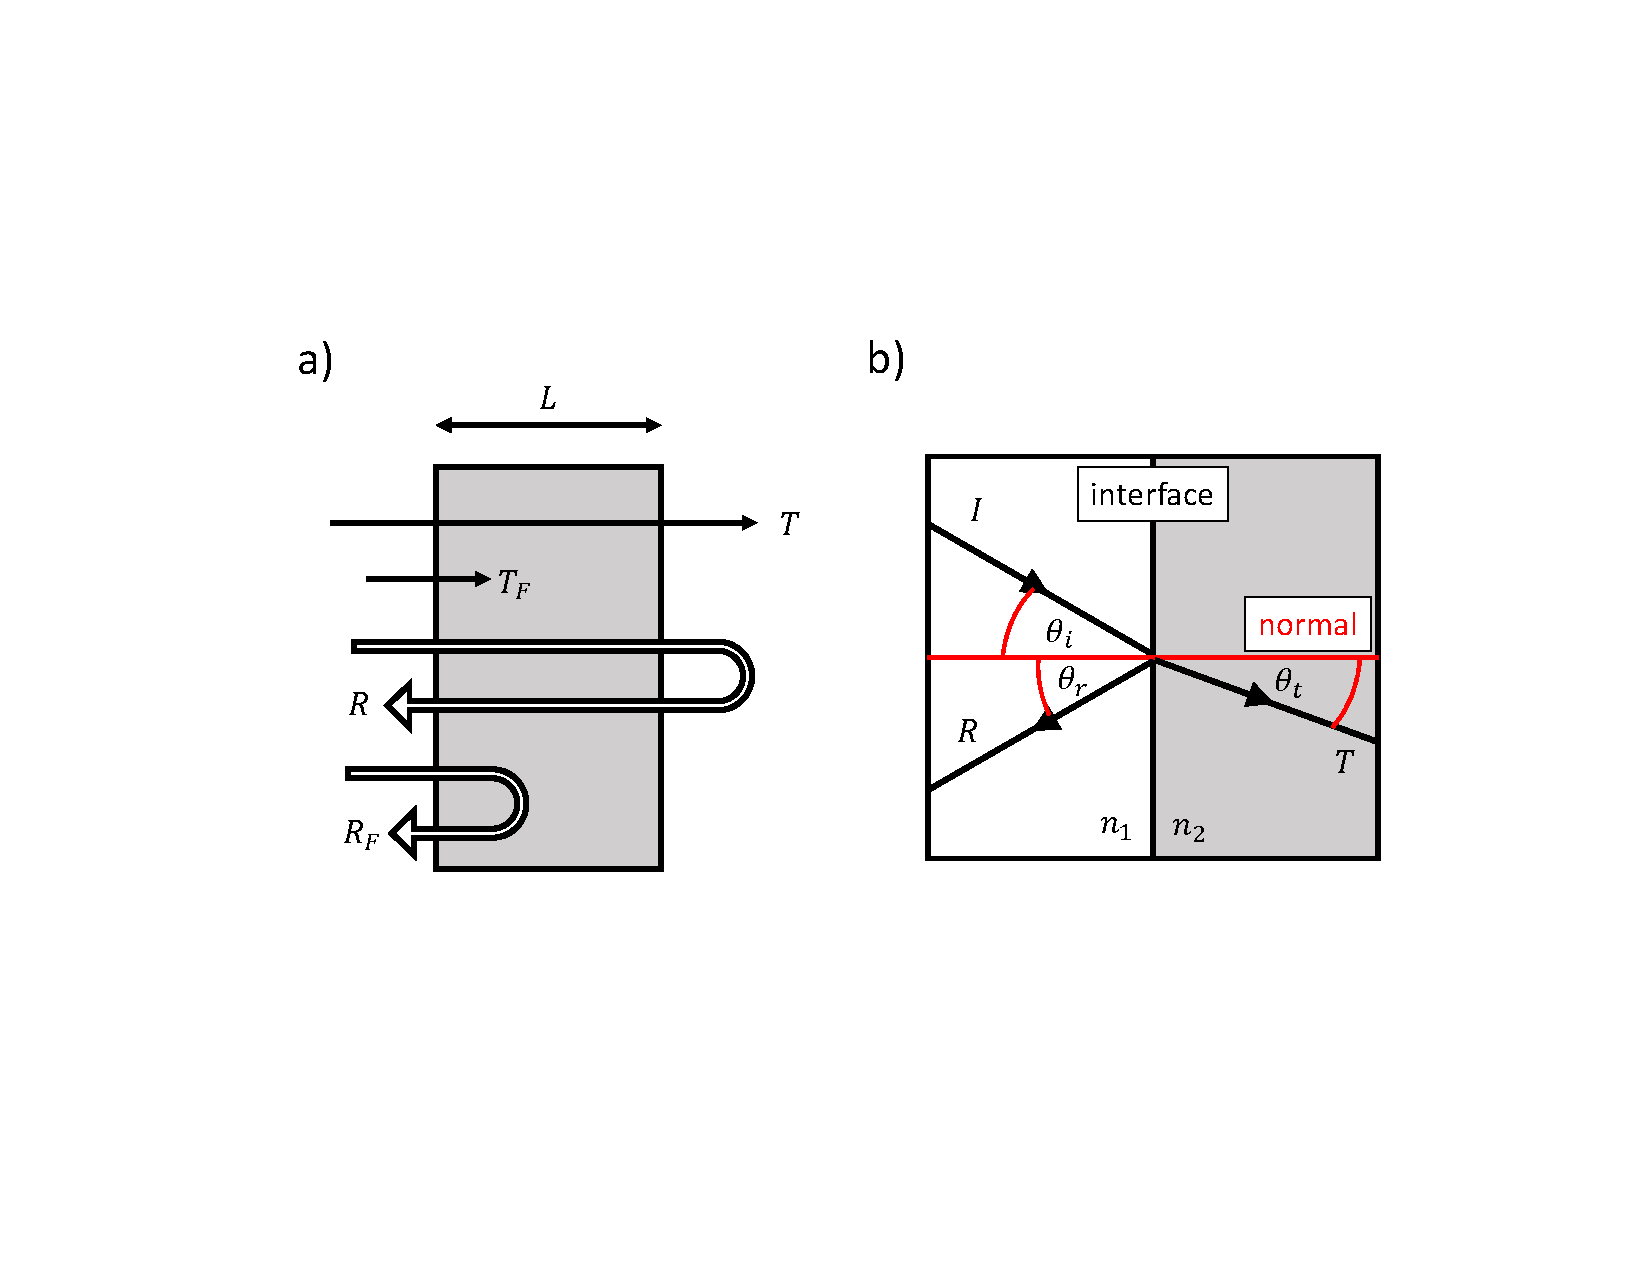
\includegraphics[width=0.75\textwidth]{figures/chap1/Fresnel_Geometry.pdf}
	\caption{Normal and non-normal incident geometries. \textbf{a)} Normal incidence geometry showing Fresnel coefficients $R_F$, $T_F$ for interfaces and total transmission $T$ and reflectance $R$ for a slab of thickness $L$. Figure recreated from \cite{nichelattiComplexRefractiveIndex2002}. \textbf{b)} Non-normal geometry showing definitions of angles $\theta_i, \theta_r$ and $\theta_t$ with respect to each interface.}
	\label{fig:Fresnel_Geometry}
\end{figure}

\begin{figure}
	\centering
	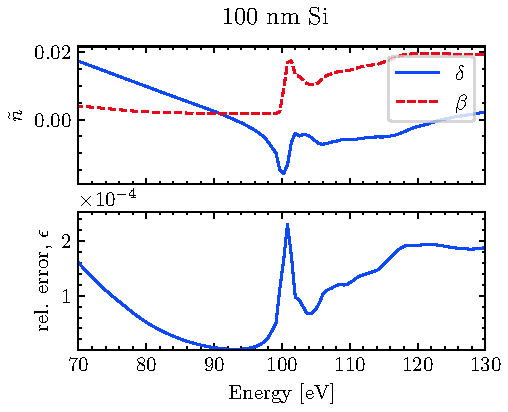
\includegraphics[width=0.75\textwidth]{figures/chap1/Si_transmission_Fresnel.pdf}
	\caption{Consequences of ignoring the real part of $\tilde{n}$ when calculating the transmission $T$ of a thin sample. Top panel: complex refractive index of silicon using the notation from \cref{eqn:complex_index}. The Si $L$-edge absorption feature is visible near 100 eV. Data from \cite{gulliksonCXROXRayInteractions}. Bottom panel: relative error in $T$, as defined in \cref{eqn:Fresnel_rel_err}, introduced by ignoring the contribution of $\Re(\tilde{n})$. An infinite number of bounces (e.g., \cref{eqn:Fresnel_coefs_inf_bounce}) is assumed.}
	\label{fig:Si_transmission_Fresnel}
	% plotted using \Python Scripts\CXRO\test\real_imag_index_plotting.py
\end{figure}

In a transient absorption experiment, we measure the transmission $T$ of a sample in response to excitation by an external field. Generally speaking, $T$ depends on both parts of the complex refractive index: $\tilde{n} = n + i k$. However, in a normal transmission geometry it turns out that the contribution of $\Im(\tilde{n})$ dominates the measured signal, and to a good approximation the role of $\Re(\tilde{n})$ can be ignored. Note that in a non-normal reflection geometry, both parts of $\tilde{n}$ make significant contributitions to the measured signal. In the following discussion we will analyze the Fresnel equations to see why this is the case. This section will draw from arguments made in reference \cite{nichelattiComplexRefractiveIndex2002}.

First, we consider the normal geometry shown in the left panel of \cref{fig:Fresnel_Geometry}. We write the complex index of refraction in the following form:
\begin{equation}
\begin{aligned}
\tilde{n} &= n - i k \\
&= (1-\delta) - i \beta
\end{aligned}
\label{eqn:complex_index}
\end{equation}
The Fresnel coefficients $R_F$ and $T_F$ describe the interface reflectance and transmittance and depend on both parts of the complex index $\tilde{n}$. For normal incidence, they are:
\begin{equation}
\begin{aligned}
R_F &= \left| \frac{n-ik-1}{n-ik+1}   \right|^2 \\
T_F &=  \frac{4n}{\left|n-ik+1\right|^2}
\end{aligned}
\label{eqn:fresnel_normal}
\end{equation}
Absorption in the bulk is described via the absorption length $\alpha$:
\begin{equation}
\alpha = 4 \pi k / \lambda
\end{equation}
Ignoring interface effects, the transmisison through the bulk is:
\begin{equation}
T_{\text{bulk}} = \exp( - \alpha L)
\end{equation}
Note that $\alpha$ and $T_{\text{bulk}}$ only depend on $k$.

The total reflectance $R$ and transmission $T$ are the result of interface effects plus bulk effects. We must consider the case where the detected light is the result of multiple reflections within the sample. Neglecting interference, we consider the case of $2N$ bounces where the laser's coherence length is less than the thickness of the bulk. In this case, the sum is incoherent with the expressions for $T$ and $R$ given by:
\begin{equation}
\begin{aligned}
R &= R_F + R_F T_F^2 T_{\text{bulk}}^2 \sum_{m=0}^{N} \left[ R_F T_{\text{bulk}} \right]^{2m} \\
T &= T_F^2 T_{\text{bulk}} \sum_{m=0}^{N} \left[ R_F T_{\text{bulk}} \right]^{2m}
\end{aligned}
\label{eqn:Fresnel_coefs_N_bounce}
\end{equation}
For the case of an infinite number of bounces, \cref{eqn:Fresnel_coefs_N_bounce} simplifies to:
\begin{equation}
\begin{aligned}
R &= R_F + \frac{R_F T_F^2 T_{\text{bulk}}^2}{1-R_F^2 T_{\text{bulk}}^2} \\
T &= \frac{T_F^2 T_{\text{bulk}}}{1-R_F^2 T_{\text{bulk}}^2},
\end{aligned}
\label{eqn:Fresnel_coefs_inf_bounce}
\end{equation}
whereas if only a single bounce occurs, \cref{eqn:Fresnel_coefs_N_bounce} reduces to:
\begin{equation}
\begin{aligned}
R &= R_F + R_F T_F^2 T_{\text{bulk}}^2 \\
T &= T_F^2 T_{\text{bulk}}
\end{aligned}
\label{eqn:Fresnel_coefs_1_bounce}
\end{equation}

We now consider the fractional error introduced by ignoring the interface effects described by $T_F$ and $R_F$. That is, what would happen if we assume that the interfaces have no effect on the transmitted intensity? We introduce the relative error $\epsilon$ made by ignoring the Fresnel coefficients of \cref{eqn:Fresnel_coefs_inf_bounce}:
\begin{equation}
\epsilon \equiv \frac{T_{\text{bulk}}}{T} - 1
\label{eqn:Fresnel_rel_err}
\end{equation}

As an example, consider a 100 nm thick Si sample measured in transmission near the Si $L$-edge (about 100 eV), as shown in \cref{fig:Si_transmission_Fresnel}. The relative error is in the range of one part in $10^4$ to $10^5$, well below our experimental detection limit. Silicon was chosen due to its data availability above and below the absorption edge, but this behavior should hold for all materials in normal transmission.

The real part of the complex index becomes important when the sample isn't normal to the beam, as shown in the right panel of \cref{fig:Fresnel_Geometry}. In this case, the Fresnel equations are a bit messier:
\begin{equation}
\begin{aligned}
R_s &= \left| \frac{\tilde{n}_1 \cos \theta_i - \tilde{n}_2 \cos \theta_t}{\tilde{n}_1 \cos \theta_i + \tilde{n}_2 \cos \theta_t}  \right|^2 \\
R_p &= \left| \frac{\tilde{n}_1 \cos \theta_t - \tilde{n}_2 \cos \theta_i}{\tilde{n}_1 \cos \theta_t + \tilde{n}_2 \cos \theta_i}  \right|^2 \\
T_s &= 1 - R_s \\
T_p &= 1 - R_p \\
%\theta_t &= \sqrt{1- \left( \frac{n_1}{n_2} \sin \theta_i \right)^2}
\end{aligned}
\label{eqn:Fresnel_nonnormal}
\end{equation}

Here, the subscripts $s$ and $p$ denote the polarization relative to the surface normal. For a sample in vacuum, $\tilde{n}_1=1$ and $\tilde{n}_2$ is the index of the sample. We can extract the relevant physics without any additional manipulation of \cref{eqn:Fresnel_nonnormal}. Right away, we can see that unlike \cref{eqn:fresnel_normal}, \cref{eqn:Fresnel_nonnormal} is symmetric in the real and imaginary parts of the sample's complex index, $\tilde{n}_2$. In the limit of a thick slab, ($L \gg \alpha$), the light is attenuated before it can reflect off the back surface and we have $T \rightarrow 0$ and $R \rightarrow R_{s,p}$. That is, the only contributions to the reflected intensity are from the interface and possibly the sample volume within $z \approx 1/\alpha$ of the interface. As a result, both parts of $\tilde{n}_2$ will make significant contributions to the reflected intensity. This geometry is common in transient reflection-absorption experiments \cite{cirriAchievingSurfaceSensitivity2017,kaplanFemtosecondTrackingCarrier2018}.



complex refractive index

sample requirements and preparation

pointing stability (in reflection, sample is an XUV optic)

\subsection{previous work}
what is state of the art?

previous work in condensed matter (Si, Ge, Si-Ge, etc)

motivation for long-wavelength studies in condensed matter

\subsection{physical observables in ATAS}
limited k-space information (requires single crystal)

transmission geometry measures imaginary and not the real part of n

\subsection{interpretation of experimental data}

\section{High Harmonic Generation (HHG)}

High harmonic generation is the process in which a strong infrared field, incident upon a medium, produces light with frequencies that are integer multiples of the fundamental field.

Gas phase HHG 

In most cases, symmetry of the light field and the generating medium leads to the suppression of even order harmonics.

symmetry leads to odd harmonics.

gas and solid HHG has been studied

\subsection{Single Atom Response}

\begin{figure}
	\centering
	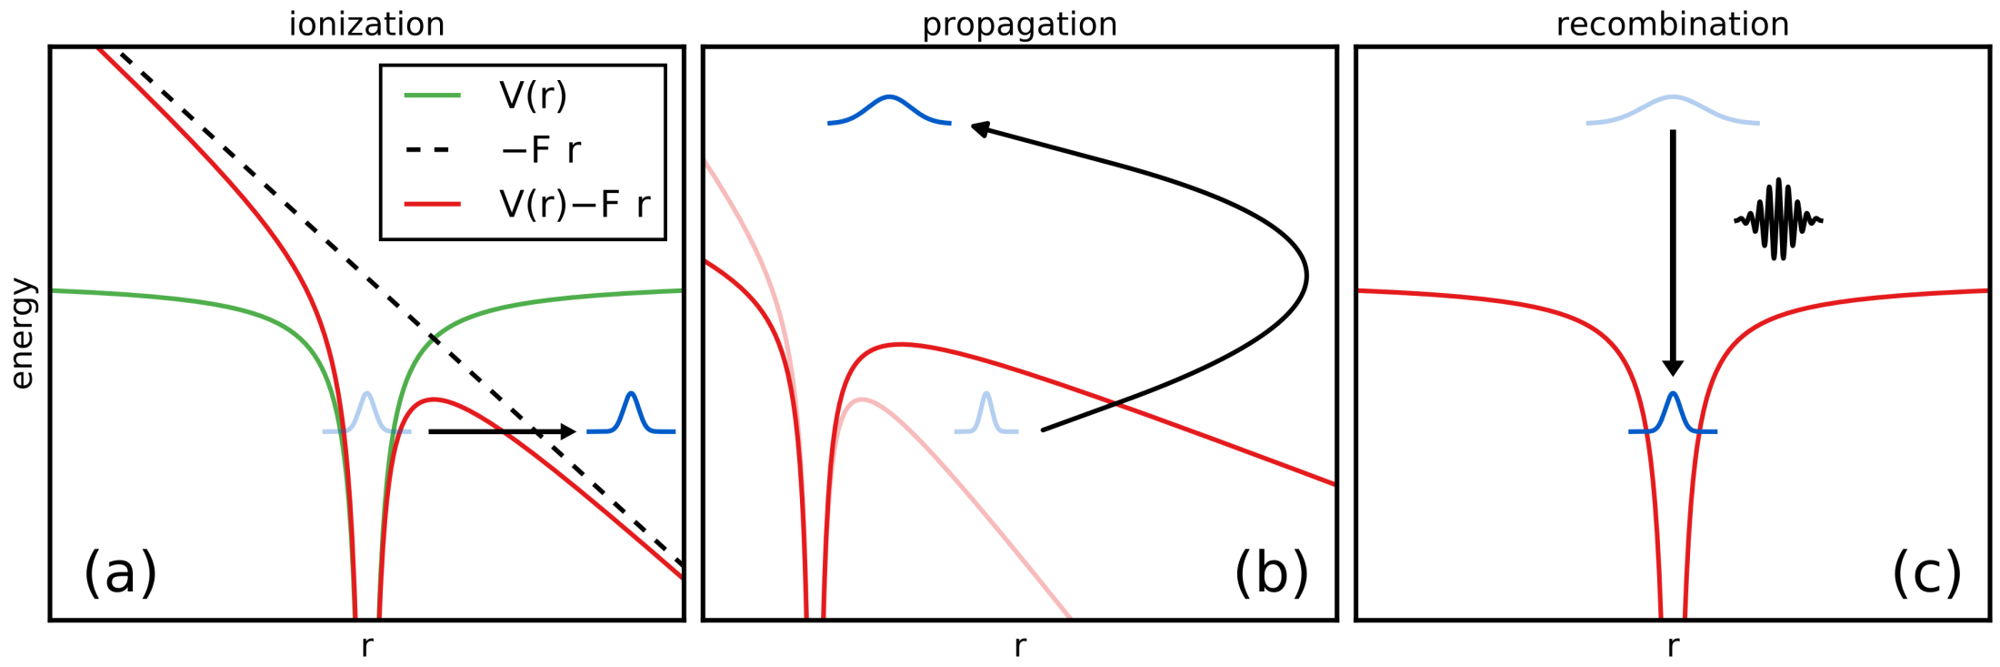
\includegraphics[width=0.75\textwidth]{figures/chap1/ThreeStepModel.png}
	\caption{3 step model from S. Schoun's thesis \cite{schounAttosecondHighHarmonicSpectroscopy2015}.}
	\label{fig:ThreeStepModel}
\end{figure}

We start with a microscopic picture of harmonic generation, focusing on the interaction between a single atom and the laser field. A semi-classical three step model has been developed to describe the process of high harmonic generation \cite{schaferThresholdIonizationHigh1993,corkumPlasmaPerspectiveStrong1993}. First, an electron is tunnel-ionized by the strong field. It is then accelerated in the field under the influence of the laser field, where it gains kinetic energy from the field. Finally, it is driven back towards the parent atom, where recombination and photoemission can occur.

\cref{fig:ThreeStepModel} shows the three steps.


cycle-averaged quiver energy

\begin{equation}
U_p = \frac{q_e^2 F_0^2}{4 m_e \omega^2} \propto I_0 \lambda^2
\label{eqn:Up}
\end{equation}

cutoff energy:

\begin{equation}
\omega_{cutoff} = I_p + 3.17 U_p
\label{eqn:cutoff}
\end{equation}

semi-classical three step model


\subsection{Phase Matching}

We now zoom out to the macroscopic picture, which encompasses the entire gas-laser interaction volume. Radiation from individual dipoles coherently sums efficiently if the wave vector mismatch $\Delta k$ of these independent dipoles is zero. The phase mismatch term can be expressed as three separate factors, each arising from distinct physical phenomena \cite{rothhardtAbsorptionlimitedPhasematchedHigh2014}:
\begin{equation}
\Delta k = \Delta k_{disp} + \Delta k_{Gouy} + \Delta k_{dipole}
\label{eqn:phase_mismatch}
\end{equation}
The first term represents the dispersion from the generating medium. It has contributions from both the neutral atoms and the free electrons:
\begin{equation}
\Delta k_{disp} = \frac{2 \pi q}{\lambda} \frac{p}{p_0} \Delta \delta \left( 1 - \frac{\eta}{\eta_c} \right)
\end{equation}
Here, $q$ is the harmonic order, $\Delta \delta$ is the difference of the refractive indices of the fundamental and high order harmonic, $p_0$ is the standard pressure (1013 mbar), $p$ is the interaction pressure, $\eta$ is the ionization fraction and $\eta_c$ is the critical ionization fraction (the fraction at which the plasma dispersion of the free electrons exceeds the atomic dispersion).

The second term is the geometrical phase mismatch caused by focusing:
\begin{equation}
\Delta k_{Gouy} = q \pdv{\varphi_{Gouy}}{z} = q \pdv{z} \left( - \arctan \left( \frac{z}{z_R} \right) \right)
\label{eqn:deltak_Gouy}
\end{equation}
Here, $z_R = \pi w_0^2 / \lambda$ is the Rayleigh range and $z=0$ corresponds to the focal plane. Note that $\Delta k_{Gouy}$ is negative for all values of $z$. The atomic term arises from the intensity-dependent dipole phase acquired during the electron excursion \cite{lewensteinTheoryHighharmonicGeneration1994,balcouGeneralizedPhasematchingConditions1997,salieresCoherenceControlHighOrder1995}:
\begin{equation}
\Delta k_{dipole} = - \alpha_q \pdv{I}{z}
\label{eqn:deltak_atomic}
\end{equation}
The value of $\alpha_q$ depends on the quantum trajectory the electron takes during its excursion. For short trajectories, {$\alpha_q = 2 \times 10^{-14}$ cm\textsuperscript{2}/W} and for long trajectories, {$\alpha_q = 22 \times 10^{-14}$ cm\textsuperscript{2}/W} \cite{kazamiasPressureinducedPhaseMatching2011,balcouQuantumpathAnalysisPhase1999}.

Note that the dispersion phase can be controlled by tuning the interaction pressure $p$, while the other terms are (to first order) pressure independent. If the gas medium is at focus, $\pdv{I}{z} = 0$ and therefore $k_{dipole}=0$. In this case, the condition $\Delta k = 0$ can be met by setting to the pressure to an optimal phase matching pressure $p_{opt}$ \cite{rothhardtAbsorptionlimitedPhasematchedHigh2014}:
\begin{equation}
p_{opt} = p_0 \frac{\lambda^2}{2 \pi^2 w_0^2 \Delta \delta \left( 1 - \frac{\eta}{\eta_c} \right)}
\label{eqn:phase_matching_pressure}
\end{equation}

We therefore arrive at the conclusion that the optimal phase matching pressure scales with the square of the fundamental wavelength. Furthermore, tighter focusing ($w_0 \rightarrow 0$) and higher ionization fractions ($\eta \rightarrow \eta_c$) require larger pressures. Thus, our vacuum system and gas source need to be able to deliver significantly higher interaction pressures when generating harmonics at long wavelengths using a weaker driving field (which requires tighter focusing).

\subsubsection{1D phase matching model}

we now consider the effects of absorption on the phase matching process.

for the $q^{th}$ harmonic, the number $N_{out}$ of photons emitted on axis per unit time and of area is proportional to \cite{constantOptimizingHighHarmonic1999}:

\begin{equation}
\rho^2 A_q^2 \frac{4L_{abs}^2}{1+4\pi^2(L_{abs}^2 / L_{coh}^2)} \left[ 1 + \exp\left(-\frac{L_{med}}{L_{abs}}\right) - 2 \exp\left(\frac{\pi L_{med}}{L_{coh}}\right) \exp\left(-\frac{L_{med}}{2L_{abs}}\right) \right]
\label{eqn:HHGNout}
\end{equation}

where $L_{coh} = \pi/\Delta k$ is the coherence length ($\Delta k = k_q - q k_0$)

